% Conditional Neural Process.  Build: latexmk -pdf cnp.tex
\documentclass[border=8pt]{standalone}
\usepackage{amsmath}
% Shared TikZ palette + node styles for the ML-RT2 architecture diagrams.
% Colours match the ML-RT comparison-paper figures so the three papers look consistent:
%   pink   = data / vectors (inputs, outputs, latent representations)
%   blue   = learned networks / operators (MLPs, encoders, decoders, ...)
%   orange = special operations / physics (spectral transforms, RT residual, ...)
%   green  = loss / training terms
\usepackage{tikz}
\usetikzlibrary{arrows.meta,positioning,fit,backgrounds,calc}

\definecolor{dataFill}{HTML}{F2E6FF}\definecolor{dataDraw}{HTML}{6600CC}
\definecolor{netFill}{HTML}{B5E8E8}\definecolor{netDraw}{HTML}{086565}
\definecolor{opFill}{HTML}{FFE0C2}\definecolor{opDraw}{HTML}{AB4F03}
\definecolor{lossFill}{HTML}{C8F4C1}\definecolor{lossDraw}{HTML}{0C5600}

\tikzset{
  font=\small,
  box/.style  ={draw, rounded corners, align=center, inner sep=4pt, minimum height=9mm, line width=0.3mm},
  data/.style ={box, fill=dataFill, draw=dataDraw},
  net/.style  ={box, fill=netFill,  draw=netDraw},
  op/.style   ={box, fill=opFill,   draw=opDraw},
  loss/.style ={box, fill=lossFill, draw=lossDraw},
  sum/.style  ={draw=netDraw, circle, inner sep=1.3pt, fill=white, line width=0.3mm},
  arr/.style  ={-{Stealth[length=2.4mm]}, thick},
  darr/.style ={-{Stealth[length=2.4mm]}, thick, dashed},
  note/.style ={align=center, font=\scriptsize, text=black!65},
}

\begin{document}
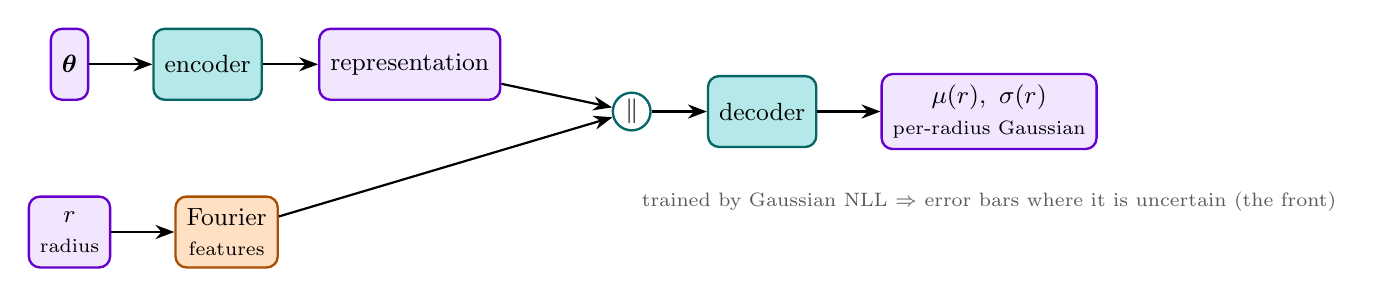
\begin{tikzpicture}
  \node[data]                      (th)  {$\boldsymbol{\theta}$};
  \node[net,  right=8mm of th]     (enc) {encoder};
  \node[data, right=7mm of enc]    (rep) {representation};
  \node[data, below=12mm of th]    (r)   {$r$\\{\scriptsize radius}};
  \node[op,   right=8mm of r]      (ff)  {Fourier\\{\scriptsize features}};
  \node[sum,  right=14mm of rep, yshift=-6mm] (cat) {$\Vert$};
  \node[net,  right=7mm of cat]    (dec) {decoder};
  \node[data, right=8mm of dec]    (out) {$\mu(r),\ \sigma(r)$\\{\scriptsize per-radius Gaussian}};

  \draw[arr] (th)--(enc); \draw[arr] (enc)--(rep);
  \draw[arr] (r)--(ff);
  \draw[arr] (rep)--(cat); \draw[arr] (ff)--(cat);
  \draw[arr] (cat)--(dec); \draw[arr] (dec)--(out);
  \node[below=4mm of out, note]
        {trained by Gaussian NLL $\Rightarrow$ error bars where it is uncertain (the front)};
\end{tikzpicture}
\end{document}
